%% This is a sample file demonstrating the use of IJCAS.cls,
%% which is for the IJCAS (International Journal of Control, Automation, and Systems).
%%
%% 2004/03/08 by Karnes Kim
%% 2011/07/26 by CDSL, SNU
%%
%% Support sites: http://www.ijcas.com
%%
%% This code is offered as-is - no warranty - user assumes all risk.
%% Free to use, distribute and modify.
%%

%% The IJCAS class supports two column page basically. 
%%So, you need not use two column option or command.
\documentclass{IJCAS}

%% include the useful LaTeX packages:
\usepackage{url}
\usepackage{array,tabularx}
\usepackage{multicol} 
\usepackage{multirow}

%%%% Editorial Information
%% Authors do not have to modify this section.
\journalvolumn{VV}
\journalnumber{X}
\journalyear{YYYY}
\setarticlestartpagenumber{1}
%%%% End of Editorial Information

%The environment for theorem, lemma, remark, corollary, proposition, and definition are already defined.


%The following command is needed for line break of long equations.
\allowdisplaybreaks


\begin{document}

\newcommand{\getErrorResult}[5]{\csname#1#2#3#4#5\endcsname}
\newcommand{\FlatodometryControllerVelerrorEstimateNormMeanabs}{0.034}
\newcommand{\FlatodometryControllerVelerrorEstimateNormStd}{0.033}
\newcommand{\FlatodometryControllerVelerrorEstimateXyMeanabs}{0.030}
\newcommand{\FlatodometryControllerVelerrorEstimateXyStd}{0.030}
\newcommand{\FlatodometryControllerVelerrorEstimateZMeanabs}{0.013}
\newcommand{\FlatodometryControllerVelerrorEstimateZStd}{0.021}
\newcommand{\FlatodometryControllerVelerrorLlveNormMeanabs}{0.034}
\newcommand{\FlatodometryControllerVelerrorLlveNormStd}{0.033}
\newcommand{\FlatodometryControllerVelerrorLlveXyMeanabs}{0.030}
\newcommand{\FlatodometryControllerVelerrorLlveXyStd}{0.030}
\newcommand{\FlatodometryControllerVelerrorLlveZMeanabs}{0.013}
\newcommand{\FlatodometryControllerVelerrorLlveZStd}{0.022}
\newcommand{\FlatodometryHartleyVelerrorEstimateNormMeanabs}{0.017}
\newcommand{\FlatodometryHartleyVelerrorEstimateNormStd}{0.015}
\newcommand{\FlatodometryHartleyVelerrorEstimateXyMeanabs}{0.015}
\newcommand{\FlatodometryHartleyVelerrorEstimateXyStd}{0.015}
\newcommand{\FlatodometryHartleyVelerrorEstimateZMeanabs}{0.006}
\newcommand{\FlatodometryHartleyVelerrorEstimateZStd}{0.009}
\newcommand{\FlatodometryHartleyVelerrorLlveNormMeanabs}{0.092}
\newcommand{\FlatodometryHartleyVelerrorLlveNormStd}{0.142}
\newcommand{\FlatodometryHartleyVelerrorLlveXyMeanabs}{0.090}
\newcommand{\FlatodometryHartleyVelerrorLlveXyStd}{0.141}
\newcommand{\FlatodometryHartleyVelerrorLlveZMeanabs}{0.011}
\newcommand{\FlatodometryHartleyVelerrorLlveZStd}{0.019}
\newcommand{\FlatodometryTiltVelerrorEstimateNormMeanabs}{0.019}
\newcommand{\FlatodometryTiltVelerrorEstimateNormStd}{0.019}
\newcommand{\FlatodometryTiltVelerrorEstimateXyMeanabs}{0.018}
\newcommand{\FlatodometryTiltVelerrorEstimateXyStd}{0.018}
\newcommand{\FlatodometryTiltVelerrorEstimateZMeanabs}{0.006}
\newcommand{\FlatodometryTiltVelerrorEstimateZStd}{0.010}
\newcommand{\FlatodometryTiltVelerrorLlveNormMeanabs}{0.044}
\newcommand{\FlatodometryTiltVelerrorLlveNormStd}{0.048}
\newcommand{\FlatodometryTiltVelerrorLlveXyMeanabs}{0.042}
\newcommand{\FlatodometryTiltVelerrorLlveXyStd}{0.047}
\newcommand{\FlatodometryTiltVelerrorLlveZMeanabs}{0.010}
\newcommand{\FlatodometryTiltVelerrorLlveZStd}{0.016}
\newcommand{\FlatodometryControllerRelerrorTiltMeanabs}{1.32}
\newcommand{\FlatodometryControllerRelerrorTiltStd}{2.06}
\newcommand{\FlatodometryControllerRelerrorTransxyMeanabs}{0.034}
\newcommand{\FlatodometryControllerRelerrorTransxyStd}{0.026}
\newcommand{\FlatodometryControllerRelerrorTranszMeanabs}{0.020}
\newcommand{\FlatodometryControllerRelerrorTranszStd}{0.045}
\newcommand{\FlatodometryControllerRelerrorYawMeanabs}{1.23}
\newcommand{\FlatodometryControllerRelerrorYawStd}{1.25}
\newcommand{\FlatodometryHartleyRelerrorTiltMeanabs}{1.00}
\newcommand{\FlatodometryHartleyRelerrorTiltStd}{1.84}
\newcommand{\FlatodometryHartleyRelerrorTransxyMeanabs}{0.046}
\newcommand{\FlatodometryHartleyRelerrorTransxyStd}{0.056}
\newcommand{\FlatodometryHartleyRelerrorTranszMeanabs}{0.026}
\newcommand{\FlatodometryHartleyRelerrorTranszStd}{0.051}
\newcommand{\FlatodometryHartleyRelerrorYawMeanabs}{0.96}
\newcommand{\FlatodometryHartleyRelerrorYawStd}{0.92}
\newcommand{\FlatodometryTiltRelerrorTiltMeanabs}{0.94}
\newcommand{\FlatodometryTiltRelerrorTiltStd}{1.97}
\newcommand{\FlatodometryTiltRelerrorTransxyMeanabs}{0.031}
\newcommand{\FlatodometryTiltRelerrorTransxyStd}{0.021}
\newcommand{\FlatodometryTiltRelerrorTranszMeanabs}{0.030}
\newcommand{\FlatodometryTiltRelerrorTranszStd}{0.046}
\newcommand{\FlatodometryTiltRelerrorYawMeanabs}{1.15}
\newcommand{\FlatodometryTiltRelerrorYawStd}{1.18}
\newcommand{\FlatodometryControllerAbserrorKoTrobobdRhpsaATiltMeanabs}{1.08}
\newcommand{\FlatodometryControllerAbserrorKoTrobobdRhpsaATiltStd}{0.43}
\newcommand{\FlatodometryControllerAbserrorKoTrobobdRhpsaATransxyMeanabs}{0.236}
\newcommand{\FlatodometryControllerAbserrorKoTrobobdRhpsaATransxyStd}{0.144}
\newcommand{\FlatodometryControllerAbserrorKoTrobobdRhpsaATranszMeanabs}{0.002}
\newcommand{\FlatodometryControllerAbserrorKoTrobobdRhpsaATranszStd}{0.003}
\newcommand{\FlatodometryControllerAbserrorKoTrobobdRhpsaAYawMeanabs}{2.71}
\newcommand{\FlatodometryControllerAbserrorKoTrobobdRhpsaAYawStd}{3.39}
\newcommand{\FlatodometryHartleyAbserrorKoTrobobdRhpsaATiltMeanabs}{1.22}
\newcommand{\FlatodometryHartleyAbserrorKoTrobobdRhpsaATiltStd}{0.40}
\newcommand{\FlatodometryHartleyAbserrorKoTrobobdRhpsaATransxyMeanabs}{0.260}
\newcommand{\FlatodometryHartleyAbserrorKoTrobobdRhpsaATransxyStd}{0.115}
\newcommand{\FlatodometryHartleyAbserrorKoTrobobdRhpsaATranszMeanabs}{0.160}
\newcommand{\FlatodometryHartleyAbserrorKoTrobobdRhpsaATranszStd}{0.178}
\newcommand{\FlatodometryHartleyAbserrorKoTrobobdRhpsaAYawMeanabs}{5.54}
\newcommand{\FlatodometryHartleyAbserrorKoTrobobdRhpsaAYawStd}{6.12}
\newcommand{\FlatodometryTiltAbserrorKoTrobobdRhpsaATiltMeanabs}{0.96}
\newcommand{\FlatodometryTiltAbserrorKoTrobobdRhpsaATiltStd}{0.31}
\newcommand{\FlatodometryTiltAbserrorKoTrobobdRhpsaATransxyMeanabs}{0.226}
\newcommand{\FlatodometryTiltAbserrorKoTrobobdRhpsaATransxyStd}{0.128}
\newcommand{\FlatodometryTiltAbserrorKoTrobobdRhpsaATranszMeanabs}{0.225}
\newcommand{\FlatodometryTiltAbserrorKoTrobobdRhpsaATranszStd}{0.253}
\newcommand{\FlatodometryTiltAbserrorKoTrobobdRhpsaAYawMeanabs}{2.52}
\newcommand{\FlatodometryTiltAbserrorKoTrobobdRhpsaAYawStd}{3.08}
\newcommand{\FlatodometryControllerAbserrorKoTrobobdRhpsaBTiltMeanabs}{0.90}
\newcommand{\FlatodometryControllerAbserrorKoTrobobdRhpsaBTiltStd}{0.46}
\newcommand{\FlatodometryControllerAbserrorKoTrobobdRhpsaBTransxyMeanabs}{0.179}
\newcommand{\FlatodometryControllerAbserrorKoTrobobdRhpsaBTransxyStd}{0.107}
\newcommand{\FlatodometryControllerAbserrorKoTrobobdRhpsaBTranszMeanabs}{0.002}
\newcommand{\FlatodometryControllerAbserrorKoTrobobdRhpsaBTranszStd}{0.003}
\newcommand{\FlatodometryControllerAbserrorKoTrobobdRhpsaBYawMeanabs}{2.28}
\newcommand{\FlatodometryControllerAbserrorKoTrobobdRhpsaBYawStd}{3.40}
\newcommand{\FlatodometryHartleyAbserrorKoTrobobdRhpsaBTiltMeanabs}{1.11}
\newcommand{\FlatodometryHartleyAbserrorKoTrobobdRhpsaBTiltStd}{0.36}
\newcommand{\FlatodometryHartleyAbserrorKoTrobobdRhpsaBTransxyMeanabs}{0.154}
\newcommand{\FlatodometryHartleyAbserrorKoTrobobdRhpsaBTransxyStd}{0.100}
\newcommand{\FlatodometryHartleyAbserrorKoTrobobdRhpsaBTranszMeanabs}{0.154}
\newcommand{\FlatodometryHartleyAbserrorKoTrobobdRhpsaBTranszStd}{0.177}
\newcommand{\FlatodometryHartleyAbserrorKoTrobobdRhpsaBYawMeanabs}{2.05}
\newcommand{\FlatodometryHartleyAbserrorKoTrobobdRhpsaBYawStd}{1.73}
\newcommand{\FlatodometryTiltAbserrorKoTrobobdRhpsaBTiltMeanabs}{0.84}
\newcommand{\FlatodometryTiltAbserrorKoTrobobdRhpsaBTiltStd}{0.30}
\newcommand{\FlatodometryTiltAbserrorKoTrobobdRhpsaBTransxyMeanabs}{0.168}
\newcommand{\FlatodometryTiltAbserrorKoTrobobdRhpsaBTransxyStd}{0.101}
\newcommand{\FlatodometryTiltAbserrorKoTrobobdRhpsaBTranszMeanabs}{0.196}
\newcommand{\FlatodometryTiltAbserrorKoTrobobdRhpsaBTranszStd}{0.228}
\newcommand{\FlatodometryTiltAbserrorKoTrobobdRhpsaBYawMeanabs}{4.18}
\newcommand{\FlatodometryTiltAbserrorKoTrobobdRhpsaBYawStd}{4.88}
\newcommand{\FlatodometryControllerAbserrorKoTrobobdRhpsaCTiltMeanabs}{1.04}
\newcommand{\FlatodometryControllerAbserrorKoTrobobdRhpsaCTiltStd}{0.48}
\newcommand{\FlatodometryControllerAbserrorKoTrobobdRhpsaCTransxyMeanabs}{0.303}
\newcommand{\FlatodometryControllerAbserrorKoTrobobdRhpsaCTransxyStd}{0.189}
\newcommand{\FlatodometryControllerAbserrorKoTrobobdRhpsaCTranszMeanabs}{0.002}
\newcommand{\FlatodometryControllerAbserrorKoTrobobdRhpsaCTranszStd}{0.003}
\newcommand{\FlatodometryControllerAbserrorKoTrobobdRhpsaCYawMeanabs}{4.72}
\newcommand{\FlatodometryControllerAbserrorKoTrobobdRhpsaCYawStd}{5.31}
\newcommand{\FlatodometryHartleyAbserrorKoTrobobdRhpsaCTiltMeanabs}{1.01}
\newcommand{\FlatodometryHartleyAbserrorKoTrobobdRhpsaCTiltStd}{0.36}
\newcommand{\FlatodometryHartleyAbserrorKoTrobobdRhpsaCTransxyMeanabs}{0.155}
\newcommand{\FlatodometryHartleyAbserrorKoTrobobdRhpsaCTransxyStd}{0.112}
\newcommand{\FlatodometryHartleyAbserrorKoTrobobdRhpsaCTranszMeanabs}{0.150}
\newcommand{\FlatodometryHartleyAbserrorKoTrobobdRhpsaCTranszStd}{0.165}
\newcommand{\FlatodometryHartleyAbserrorKoTrobobdRhpsaCYawMeanabs}{3.05}
\newcommand{\FlatodometryHartleyAbserrorKoTrobobdRhpsaCYawStd}{3.30}
\newcommand{\FlatodometryTiltAbserrorKoTrobobdRhpsaCTiltMeanabs}{0.76}
\newcommand{\FlatodometryTiltAbserrorKoTrobobdRhpsaCTiltStd}{0.32}
\newcommand{\FlatodometryTiltAbserrorKoTrobobdRhpsaCTransxyMeanabs}{0.203}
\newcommand{\FlatodometryTiltAbserrorKoTrobobdRhpsaCTransxyStd}{0.104}
\newcommand{\FlatodometryTiltAbserrorKoTrobobdRhpsaCTranszMeanabs}{0.191}
\newcommand{\FlatodometryTiltAbserrorKoTrobobdRhpsaCTranszStd}{0.214}
\newcommand{\FlatodometryTiltAbserrorKoTrobobdRhpsaCYawMeanabs}{3.19}
\newcommand{\FlatodometryTiltAbserrorKoTrobobdRhpsaCYawStd}{3.78}
\newcommand{\FlatodometryControllerAbserrorKoTrobobdRhpsaDTiltMeanabs}{14.36}
\newcommand{\FlatodometryControllerAbserrorKoTrobobdRhpsaDTiltStd}{0.61}
\newcommand{\FlatodometryControllerAbserrorKoTrobobdRhpsaDTransxyMeanabs}{0.401}
\newcommand{\FlatodometryControllerAbserrorKoTrobobdRhpsaDTransxyStd}{0.367}
\newcommand{\FlatodometryControllerAbserrorKoTrobobdRhpsaDTranszMeanabs}{0.002}
\newcommand{\FlatodometryControllerAbserrorKoTrobobdRhpsaDTranszStd}{0.003}
\newcommand{\FlatodometryControllerAbserrorKoTrobobdRhpsaDYawMeanabs}{5.59}
\newcommand{\FlatodometryControllerAbserrorKoTrobobdRhpsaDYawStd}{7.47}
\newcommand{\FlatodometryHartleyAbserrorKoTrobobdRhpsaDTiltMeanabs}{13.18}
\newcommand{\FlatodometryHartleyAbserrorKoTrobobdRhpsaDTiltStd}{0.53}
\newcommand{\FlatodometryHartleyAbserrorKoTrobobdRhpsaDTransxyMeanabs}{0.300}
\newcommand{\FlatodometryHartleyAbserrorKoTrobobdRhpsaDTransxyStd}{0.256}
\newcommand{\FlatodometryHartleyAbserrorKoTrobobdRhpsaDTranszMeanabs}{0.162}
\newcommand{\FlatodometryHartleyAbserrorKoTrobobdRhpsaDTranszStd}{0.183}
\newcommand{\FlatodometryHartleyAbserrorKoTrobobdRhpsaDYawMeanabs}{11.91}
\newcommand{\FlatodometryHartleyAbserrorKoTrobobdRhpsaDYawStd}{12.38}
\newcommand{\FlatodometryTiltAbserrorKoTrobobdRhpsaDTiltMeanabs}{13.71}
\newcommand{\FlatodometryTiltAbserrorKoTrobobdRhpsaDTiltStd}{0.26}
\newcommand{\FlatodometryTiltAbserrorKoTrobobdRhpsaDTransxyMeanabs}{0.282}
\newcommand{\FlatodometryTiltAbserrorKoTrobobdRhpsaDTransxyStd}{0.209}
\newcommand{\FlatodometryTiltAbserrorKoTrobobdRhpsaDTranszMeanabs}{0.212}
\newcommand{\FlatodometryTiltAbserrorKoTrobobdRhpsaDTranszStd}{0.243}
\newcommand{\FlatodometryTiltAbserrorKoTrobobdRhpsaDYawMeanabs}{3.62}
\newcommand{\FlatodometryTiltAbserrorKoTrobobdRhpsaDYawStd}{4.01}
\newcommand{\FlatodometryControllerAbserrorKoTrobobdRhpsaETiltMeanabs}{1.82}
\newcommand{\FlatodometryControllerAbserrorKoTrobobdRhpsaETiltStd}{0.52}
\newcommand{\FlatodometryControllerAbserrorKoTrobobdRhpsaETransxyMeanabs}{0.238}
\newcommand{\FlatodometryControllerAbserrorKoTrobobdRhpsaETransxyStd}{0.122}
\newcommand{\FlatodometryControllerAbserrorKoTrobobdRhpsaETranszMeanabs}{0.003}
\newcommand{\FlatodometryControllerAbserrorKoTrobobdRhpsaETranszStd}{0.003}
\newcommand{\FlatodometryControllerAbserrorKoTrobobdRhpsaEYawMeanabs}{2.77}
\newcommand{\FlatodometryControllerAbserrorKoTrobobdRhpsaEYawStd}{2.01}
\newcommand{\FlatodometryHartleyAbserrorKoTrobobdRhpsaETiltMeanabs}{0.57}
\newcommand{\FlatodometryHartleyAbserrorKoTrobobdRhpsaETiltStd}{0.46}
\newcommand{\FlatodometryHartleyAbserrorKoTrobobdRhpsaETransxyMeanabs}{0.205}
\newcommand{\FlatodometryHartleyAbserrorKoTrobobdRhpsaETransxyStd}{0.104}
\newcommand{\FlatodometryHartleyAbserrorKoTrobobdRhpsaETranszMeanabs}{0.147}
\newcommand{\FlatodometryHartleyAbserrorKoTrobobdRhpsaETranszStd}{0.171}
\newcommand{\FlatodometryHartleyAbserrorKoTrobobdRhpsaEYawMeanabs}{4.26}
\newcommand{\FlatodometryHartleyAbserrorKoTrobobdRhpsaEYawStd}{4.55}
\newcommand{\FlatodometryTiltAbserrorKoTrobobdRhpsaETiltMeanabs}{1.21}
\newcommand{\FlatodometryTiltAbserrorKoTrobobdRhpsaETiltStd}{0.24}
\newcommand{\FlatodometryTiltAbserrorKoTrobobdRhpsaETransxyMeanabs}{0.197}
\newcommand{\FlatodometryTiltAbserrorKoTrobobdRhpsaETransxyStd}{0.092}
\newcommand{\FlatodometryTiltAbserrorKoTrobobdRhpsaETranszMeanabs}{0.203}
\newcommand{\FlatodometryTiltAbserrorKoTrobobdRhpsaETranszStd}{0.232}
\newcommand{\FlatodometryTiltAbserrorKoTrobobdRhpsaEYawMeanabs}{2.44}
\newcommand{\FlatodometryTiltAbserrorKoTrobobdRhpsaEYawStd}{2.37}



\newcommand{\MulticontactControllerVelerrorEstimateNormMeanabs}{0.034}
\newcommand{\MulticontactControllerVelerrorEstimateNormStd}{0.033}
\newcommand{\MulticontactControllerVelerrorEstimateXyMeanabs}{0.030}
\newcommand{\MulticontactControllerVelerrorEstimateXyStd}{0.030}
\newcommand{\MulticontactControllerVelerrorEstimateZMeanabs}{0.013}
\newcommand{\MulticontactControllerVelerrorEstimateZStd}{0.021}
\newcommand{\MulticontactControllerVelerrorLlveNormMeanabs}{0.034}
\newcommand{\MulticontactControllerVelerrorLlveNormStd}{0.033}
\newcommand{\MulticontactControllerVelerrorLlveXyMeanabs}{0.030}
\newcommand{\MulticontactControllerVelerrorLlveXyStd}{0.030}
\newcommand{\MulticontactControllerVelerrorLlveZMeanabs}{0.013}
\newcommand{\MulticontactControllerVelerrorLlveZStd}{0.022}
\newcommand{\MulticontactHartleyVelerrorEstimateNormMeanabs}{0.017}
\newcommand{\MulticontactHartleyVelerrorEstimateNormStd}{0.015}
\newcommand{\MulticontactHartleyVelerrorEstimateXyMeanabs}{0.015}
\newcommand{\MulticontactHartleyVelerrorEstimateXyStd}{0.015}
\newcommand{\MulticontactHartleyVelerrorEstimateZMeanabs}{0.006}
\newcommand{\MulticontactHartleyVelerrorEstimateZStd}{0.009}
\newcommand{\MulticontactHartleyVelerrorLlveNormMeanabs}{0.092}
\newcommand{\MulticontactHartleyVelerrorLlveNormStd}{0.142}
\newcommand{\MulticontactHartleyVelerrorLlveXyMeanabs}{0.090}
\newcommand{\MulticontactHartleyVelerrorLlveXyStd}{0.141}
\newcommand{\MulticontactHartleyVelerrorLlveZMeanabs}{0.011}
\newcommand{\MulticontactHartleyVelerrorLlveZStd}{0.019}
\newcommand{\MulticontactTiltVelerrorEstimateNormMeanabs}{0.019}
\newcommand{\MulticontactTiltVelerrorEstimateNormStd}{0.019}
\newcommand{\MulticontactTiltVelerrorEstimateXyMeanabs}{0.018}
\newcommand{\MulticontactTiltVelerrorEstimateXyStd}{0.018}
\newcommand{\MulticontactTiltVelerrorEstimateZMeanabs}{0.006}
\newcommand{\MulticontactTiltVelerrorEstimateZStd}{0.010}
\newcommand{\MulticontactTiltVelerrorLlveNormMeanabs}{0.044}
\newcommand{\MulticontactTiltVelerrorLlveNormStd}{0.048}
\newcommand{\MulticontactTiltVelerrorLlveXyMeanabs}{0.042}
\newcommand{\MulticontactTiltVelerrorLlveXyStd}{0.047}
\newcommand{\MulticontactTiltVelerrorLlveZMeanabs}{0.010}
\newcommand{\MulticontactTiltVelerrorLlveZStd}{0.016}
\newcommand{\MulticontactControllerRelerrorTiltMeanabs}{1.16}
\newcommand{\MulticontactControllerRelerrorTiltStd}{0.58}
\newcommand{\MulticontactControllerRelerrorTransxyMeanabs}{0.016}
\newcommand{\MulticontactControllerRelerrorTransxyStd}{0.008}
\newcommand{\MulticontactControllerRelerrorTranszMeanabs}{0.006}
\newcommand{\MulticontactControllerRelerrorTranszStd}{0.007}
\newcommand{\MulticontactControllerRelerrorYawMeanabs}{0.50}
\newcommand{\MulticontactControllerRelerrorYawStd}{0.35}
\newcommand{\MulticontactHartleyRelerrorTiltMeanabs}{0.57}
\newcommand{\MulticontactHartleyRelerrorTiltStd}{1.02}
\newcommand{\MulticontactHartleyRelerrorTransxyMeanabs}{0.012}
\newcommand{\MulticontactHartleyRelerrorTransxyStd}{0.016}
\newcommand{\MulticontactHartleyRelerrorTranszMeanabs}{0.004}
\newcommand{\MulticontactHartleyRelerrorTranszStd}{0.007}
\newcommand{\MulticontactHartleyRelerrorYawMeanabs}{0.47}
\newcommand{\MulticontactHartleyRelerrorYawStd}{0.65}
\newcommand{\MulticontactTiltRelerrorTiltMeanabs}{0.23}
\newcommand{\MulticontactTiltRelerrorTiltStd}{0.17}
\newcommand{\MulticontactTiltRelerrorTransxyMeanabs}{0.007}
\newcommand{\MulticontactTiltRelerrorTransxyStd}{0.005}
\newcommand{\MulticontactTiltRelerrorTranszMeanabs}{0.002}
\newcommand{\MulticontactTiltRelerrorTranszStd}{0.003}
\newcommand{\MulticontactTiltRelerrorYawMeanabs}{0.40}
\newcommand{\MulticontactTiltRelerrorYawStd}{0.32}
\newcommand{\MulticontactControllerAbserrorHrpeMulticontactATiltMeanabs}{0.99}
\newcommand{\MulticontactControllerAbserrorHrpeMulticontactATiltStd}{0.67}
\newcommand{\MulticontactControllerAbserrorHrpeMulticontactATransxyMeanabs}{0.019}
\newcommand{\MulticontactControllerAbserrorHrpeMulticontactATransxyStd}{0.008}
\newcommand{\MulticontactControllerAbserrorHrpeMulticontactATranszMeanabs}{0.004}
\newcommand{\MulticontactControllerAbserrorHrpeMulticontactATranszStd}{0.005}
\newcommand{\MulticontactControllerAbserrorHrpeMulticontactAYawMeanabs}{1.36}
\newcommand{\MulticontactControllerAbserrorHrpeMulticontactAYawStd}{0.74}
\newcommand{\MulticontactHartleyAbserrorHrpeMulticontactATiltMeanabs}{0.68}
\newcommand{\MulticontactHartleyAbserrorHrpeMulticontactATiltStd}{0.26}
\newcommand{\MulticontactHartleyAbserrorHrpeMulticontactATransxyMeanabs}{0.006}
\newcommand{\MulticontactHartleyAbserrorHrpeMulticontactATransxyStd}{0.003}
\newcommand{\MulticontactHartleyAbserrorHrpeMulticontactATranszMeanabs}{0.003}
\newcommand{\MulticontactHartleyAbserrorHrpeMulticontactATranszStd}{0.003}
\newcommand{\MulticontactHartleyAbserrorHrpeMulticontactAYawMeanabs}{1.35}
\newcommand{\MulticontactHartleyAbserrorHrpeMulticontactAYawStd}{0.67}
\newcommand{\MulticontactTiltAbserrorHrpeMulticontactATiltMeanabs}{0.34}
\newcommand{\MulticontactTiltAbserrorHrpeMulticontactATiltStd}{0.17}
\newcommand{\MulticontactTiltAbserrorHrpeMulticontactATransxyMeanabs}{0.009}
\newcommand{\MulticontactTiltAbserrorHrpeMulticontactATransxyStd}{0.003}
\newcommand{\MulticontactTiltAbserrorHrpeMulticontactATranszMeanabs}{0.004}
\newcommand{\MulticontactTiltAbserrorHrpeMulticontactATranszStd}{0.005}
\newcommand{\MulticontactTiltAbserrorHrpeMulticontactAYawMeanabs}{1.06}
\newcommand{\MulticontactTiltAbserrorHrpeMulticontactAYawStd}{0.93}


% the \title command
\title{VALINOR: a lightweight leg inertial odometry for humanoid robots}

% the \author command
% the \orcid{orcid number}
\author{Arnaud Demont*\orcid{https://orcid.org/0009-0006-8325-8331}, Mehdi Benallegue\orcid{https://orcid.org/0000-0001-7537-9498}, and Abdelaziz Benallegue\orcid{}}

% the abstract environment
\begin{abstract}
This article describes the preparation procedure for publication in the International Journal of Control, Automation, and Systems (IJCAS), and this template applies both for initial submission and the final camera-ready manuscript of the paper. When authors submit their work for review, it is necessary to follow these instructions. The abstract should not exceed 300 words for regular papers or 75 words for technical notes and correspondence without equations, references, and footnotes.
\end{abstract}

\begin{keywords}
  Legged robots, proprioceptive odometry, state estimation, tilt estimation.
\end{keywords}

\maketitle

\makeAuthorInformation{
% Manuscript received January 10, 2025; revised March 10, 2025; accepted May 10, 2025. Recommended by Associate Editor Soon-Shin Lee under the direction of Editor Milton John.\\
A. Demont, M. Benallegue and A. Benallegue are with the CNRS-AIST JRL (Joint Robotics Laboratory), IRL, National Institute of Advanced Industrial Science and Technology (AIST), 1-1-1 Umezono, Tsukuba, Ibaraki 305-8560 Japan. 

A. Demont and A. Benallegue are also with Université Paris-Saclay, 3 rue Joliot Curie, Bâtiment Breguet, 91190 Gif-sur-Yvette, France, and Laboratoire d'Ingénierie des Systèmes de Versailles, 10-12 avenue de l'Europe, 78140 Vélizy, France. 

e-mails: arnaud.demont@aist.go.jp, mehdi.benallegue@aist.go.jp, abdelaziz.benallegue@uvsq.fr.

* Corresponding author.
}

\runningtitle{2025}{Arnaud Demont, Mehdi Benallegue and Abdelaziz Benallegue}{Manuscript Template for the International Journal of Control, Automation, and Systems: ICROS {\&} KIEE}{xxx}{xxxx}{x}




\section{INTRODUCTION}




The control of humanoid robots is a very challenging topic. As under-actuated systems, these robots have to apply reaction forces at contacts with their environment in order to generate a desired trajectory. This implies strict constraints on the center of pressure of contacts for a motion to be achievable while ensuring stability. The position of these centers of pressure must therefore be estimated along with the kinematics of the robot to predict its dynamics. This is generally done by estimating the pose and velocity of the humanoid robot's floating base. Indeed, from these variables and the reading of joint encoders, one can reconstruct the full body configuration of the robot in the world frame.

\subsection{Related Works}
    To ensure a reliable control, the pose of the floating base must be estimated at very high frequency. To this end, one commonly performs inertial odometry \textcolor{red}{buchanan2022LearningInertialOdometry} by integrating the signals provided by IMUs, composed of an accelerometer and a gyrometer, that respectively measure the angular velocity and the linear acceleration (including the gravitational acceleration) of the sensor in the world frame, expressed in the frame of the sensor. However, using only these sensors, the position, linear velocity and the yaw in the world frame are non-observable. They will therefore be subject to drift at low frequency due to the integration of the sensor noises. 
    A widely adopted solution to deal with the drift inherent in the inertial odometry is to combine it with a legged odometry \textcolor{red}{Citer}, that uses the contacts that the robot successively creates with the environment as fixed points in the environment, constraining the kinematics \textcolor{red}{bloesch2013state}. Using the joint encoders, the legged odometry provides an estimate of the position at low frequency and prevents the drift. However, this method relies on the assumption that there is no slippage between the robot and the environment at the contact. In addition, it highly depends on the accuracy of the estimated pose of the contact at the time it is considered as fixed, and thus it depends on the compliance of the robot, the contact detection framework, etc. This combination of the inertial and legged odometry methods is the most common example of \emph{dead reckoning} \textcolor{red}{roston1991deadReckoning} in the literature, a term that more generally refers to any approach based on proprioceptive sensors. Dead reckoning is a satisfactory solution for tasks that don't require a perfect knowledge of the position and yaw in the world frame, for example for some tele-operation tasks and stabilization. The latter notably relies on the estimation of the tilt of the robot, which is partially observable using the accelerometer measurement. Work has therefore been done to improve this estimation. At first obtained by considering the linear acceleration negligible with respect to the gravitational acceleration \textcolor{red}{mahony2008nonlinear}, it also took benefit from the legged odometry, the constraint on the contact allowing for a better dissociation between linear motions and the orientation \textcolor{red}{Rephrase?}. Further works focused on \textcolor{red}{Continue} or with some enhanced methods \textcolor{red}{benallegue2017tilt}. \textcolor{red}{In our work, we propose to enrich our legged odometry with the orientation of contacts. These orientations are integrated to our attitude estimator to correct the estimated yaw of the robot at low frequency, similarly to their position.}
    \textcolor{red}{legged odometry using contact orientations: ramadoss2022wholebodyKineLieKF}
    
    However, knowing these absolute kinematics is mandatory for other tasks, notably when an autonomous behaviour of the robot is desired. 
    
    To make the absolute pose of the robot observable, exteroceptive sensors, like LiDARs, cameras, etc., can be added to the estimation. The information provided by these sensors is extremely valuable, but is available only at low frequency and require a high computation capability. Also, similarly to the legged odometry failing under the slippage of contacts or with bad contact estimations, these methods can provide outliers. Known reasons can be a low illumination of the environments, low-textured environments, occlusion of the sensors, etc. The legged odometry and exteroceptive measurements therefore have complementary advantages and cons, the challenge addressed by most of the recent estimation methods is to improve the fusion between both.
    

    \textcolor{red}{To cite: Invariant Smoother for Legged Robot State 	Estimation With Dynamic Contact Event Information (they ignore contacts with too high velocity?)}
   
\subsection{Motivation}
    
As autonomous systems continue to evolve in complexity and capability, the computational demands of their decision-making processes are increasing significantly. Advanced control strategies such as Model Predictive Control (MPC) \textcolor{red}{Katayama2023MpcLeggedHumanoid, Dantec2022WholeBodyMPCTorqueControl, Dallard2024AdiosStabilizers}, reinforcement learning-based controllers \textcolor{red}{Peters2003ReinforcmentLearningForHumanoid, Li2025RLVersatileDynamicRobustBipedalLocom}, and foundation model-guided policies \textcolor{red}{"Bjorck2025GrootN1", kawaharazuka2024RealWorldApplicationsFoundationModels} are becoming more prevalent due to their ability to handle high-dimensional dynamics, long-horizon planning, and unstructured environments. However, these benefits come at the cost of heightened computational complexity, often pushing the limits of what can be executed in real time on onboard processors\textcolor{red}{"On real-time robust model predictive control", "COMPUTATIONAL DELAY IN NONLINEAR MODEL
PREDICTIVE CONTROL", "Thodoroff2022BenchmarkingRealTimeRL", "Firoozi2025FoundationModelsInRobotics"}.

As these control methods grow in computational cost, running them on resource-limited platforms like drones or embedded systems becomes a challenge. Since the control part is getting heavier, one practical solution is to reduce the computational load of other parts of the pipeline, for example the state estimation part.

State estimation remains a cornerstone of robust control, providing the essential feedback required for planning and control to operate effectively. Recognizing this trade-off, we propose an approach focused on reducing the runtime demands of the state estimator, aiming for a better balance between estimation accuracy and computational efficiency. This way, more processing time can be allocated to the increasingly demanding control algorithms without compromising the overall performance of the system.


\textcolor{red}{
As one can imagine, a slight error on the estimation of the yaw of the robot can lead to non negligible errors on the translation estimation. Therefore, estimating it as best as possible is a major objective in state estimation. The use of exteroceptive sensors is a direct solution to this issue, however they still don't offer a perfect odometry even with the most advanced methods (ex factor graphs with vilens), notably in some scenarios (ex: no loop closure, long tunnels for lidar, low-textured / low illumination environments, etc.). We propose a new orientation sensor that offers a very accurate and reliable measurement, even in challenging scenarios mentionned previously (eg: low-textured / low illumination environments), and at higher frequency (is it really much higher?). This sensor relies on a very lightweight algorithm, and can thus be used along other computationally expensive algorithms (ex: SLAM). In this article, we use this new sensor in pair with a highly accurate tilt estimation as inputs for a basic legged odometry. The purpose of this is to show how improved the legged odometry is with our orientation measurement even in a naive estimation framework unaware of information coupling, etc., to highlight the interest to include it  to more sophisticated ones (that most of the time just add combine the legged odometry with other sensors in the most effective way possible).}
    
    LOSELY COUPLED (don't forget that we are losely coupled)
    TIGHTLY COUPLED

    While working on a basic legged odometry implementation, we noticed that the main source of error in the estimation was the yaw, which is highly subject to drifts while turning. Over long translations, the erroneous yaw leads to drastic errors on the absolute position estimation. We aim to correct this by using a novel orientation measurement. CONTINUER.
    We propose a legged odometry based on a very accurate tilt estimation, allowing for a good contact estimation along translations, and on a very accurate yaw orientation.

    \textcolor{red}{Possible use case: spatial exploration}




\subsection{Contributions}
\begin{itemize}
  \item Presentation of axis agnostic orientation combinations.
  \item Lightweight combination of Leg Odometry with a highly accurate tilt estimate.
  \item Experimental evaluation of the Tilt Observer.
\end{itemize}

\section{Preliminaries}

\subsection{General notations}
\begin{itemize}
    \item The general notation for kinematic variables is $^{1}\bigcirc_{2}$ , expressing the kinematics of the frame $2$ in the frame $1$. To simplify the notation, kinematics in the world frame are written without the $\mathcal{W}$ symbol: $^{\mathcal{W}}\bigcirc_{2}=\bigcirc_{2}$.
    \item We define $\boldsymbol{\Omega}$ the function that associates the rotation matrix to the corresponding rotation vector:
    \begin{flalign}
          \text{SO}\!\left(3\right) & \rightarrow \mathbb{R}^{3}                 && \\
         \Omega: \boldsymbol{R} & \mapsto \boldsymbol{v}, \;\;\;\; \text{s.t.} \;\;\; \text{exp}\! \left(\text{S}\!\left( \boldsymbol{v} \right) \right) = \boldsymbol{R}  \text{    and    } \left| \boldsymbol{v} \right| \leq \pi     && \label{eq:Omega}
    \end{flalign}
    \item \textcolor{red}{Define vec }
    \item The world frame and the robot's IMU frame are denoted $\mathcal{W}$ and $\mathcal{I}$, respectively. The frame associated with the $i$-th contact is denoted $\mathcal{C}_{i}$. The anchor point, defined in Section~\ref{}, is denoted $\mathcal{A}$. 
    \item We define $n_c$ the number of current contacts set with the environment.
    
\end{itemize} 

\section{Axis agnostic orientation combinations}
Use of the axis agnostic representation to merge orientations

\section{Definition of the Anchor Point}
\textcolor{red}{define rest frames. I already talk about the fixed contacts right after so adapt it.}
\textcolor{red}{J'essaie de n'avoir qu'un repere pour les contacts, donc pas de repos}
We define here the notion of anchor point, since it will be used extensively in the following sections. The anchor point, denoted $\mathcal{A}$, is a point attached to the robot, and which is considered to have a zero velocity in the world frame. As will be explained in Section\textcolor{red}{sec}, this frame is especially important, since it provides a measurement of the robot's IMU velocity in the world frame. In the case of legged robots, it is common to assume that contacts with the environment are fixed. Any point of a contact surface would thus be usable as an anchor point. However, in order to pick a unique point that remains valid as contacts are created and broken, and which respects as best as possible the zero-velocity criterion, we compute its kinematics through a weighted average of the kinematics of the current contact reference frames. This is shown in Figure~\ref{fig:anchorFrame}. \\
The $i$-th contact's weighting coefficient $\lambda_{i}$ is defined as the ratio of its measured reaction force $\boldsymbol{F}_{i}$ to the total reaction force across all contacts: $\lambda_{i}=\frac{\boldsymbol{F}_{i}}{\sum^{n_{c}}_{j=1}\boldsymbol{F}_{j}}$. \\ 
As a contact weakens, its reaction force decreases, reducing its influence on the anchor point's kinematics. This helps mitigate slippage, since weaker contacts are more likely to violate Coulomb's assumption and slip. It is important to note that although the anchor point is defined to have zero velocity in the world, its pose may still evolve over time. \textcolor{red}{In discrete time, it has zero velocity? Maybe such a definition helps getting rid of the additional frame which coincides with it.}

\begin{figure}[!t]
\begin{center}
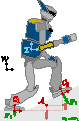
\includegraphics[width=0.5\columnwidth]{Uploaded/Images/framesAndAnchor.pdf} 
\vskip -0.5pc
\caption{Illustration of the anchor point position computation and of the reference frames used in Valinor. $\mathcal{W}$: world frame; $\mathcal{I}$: IMU frame; $\mathcal{C}_{i}$: frame of the $i$-th contact. For clarity, only the weighted average of the contact positions is shown. In this example, $\boldsymbol{F}_{2} = 2\boldsymbol{F}_{1}$, yielding a weight of $\lambda{2} = \frac{2}{3}$.}\label{fig:framesAndAnchor}
\end{center}
\vskip -1.5pc
\end{figure}

Based on this definition, we give the position and linear velocity of the anchor point in the IMU's frame, and its position in the world frame:
\begin{align} 
&{^{\mathcal{I}}}\boldsymbol{p}_{\mathcal{A}} = \sum^{n_{c}}_{i} \lambda_{i}  {^{\mathcal{I}}} \boldsymbol{p}_{{\mathcal{C}}_{i}}, \label{eq:imuAnchorPos} \\
&{^{\mathcal{I}}} \dot{\boldsymbol{p}}_{\mathcal{A}^{\prime}} = \sum^{n_{c}}_{i} \lambda_{i}  {^{\mathcal{I}}} \dot{\boldsymbol{p}}_{{\mathcal{C}}_{i}}, \label{eq:imuAnchorVel} \\
&\boldsymbol{p}_{\mathcal{A}} = \sum^{n_{c}}_{i} \lambda_{i} \boldsymbol{p}^{\star}_{{\mathcal{C}}_{i}}, \label{eq:anchorPointPos}
\end{align} 
with ${^{\mathcal{I}}} \boldsymbol{p}_{{\mathcal{C}}_{i}}$ the position and ${^{\mathcal{I}}} \dot{\boldsymbol{p}}_{{\mathcal{C}}_{i}}$ the linear velocity of the $i$-th contact in the IMU's frame, which are directly provided by the robot's joint encoders. $\boldsymbol{p}^{\star}_{{\mathcal{C}}_{i}}$ is the constant reference position of the $i$-th contact, which was its position at the instant it was created.
\textcolor{red}{What about p star and R star for the reference pose of the contacts? So we make clear they are different. But when should I talk about the reference pose of contacts? before or after ? Right above i talk about the fixed contact assumption.}
\textcolor{red}{Remove $\mathcal{A}^\prime$?}


\textcolor{red}{TODO}

\section{Tilt Observer with proof of convergence}
The proposed estimator relies on a highly accurate estimate of the IMU's tilt provided by a complementary filter, introduced in a previous work \textcolor{red}{citer}, which we will call \emph{Tilt Observer}. The Tilt Observer is a complementary filter, which based .

\subsection{Definition of the State Vector}

\subsection{Definition of the Measurements}
Let us denote $\boldsymbol{\omega}_{\mathcal{I}, l} \triangleq \boldsymbol{R}^{T}_{\mathcal{I}} \boldsymbol{\omega}_{\mathcal{I}} $ and $\boldsymbol{v}_{\mathcal{I}, l} \triangleq \boldsymbol{R}^{T}_{\mathcal{I}} \boldsymbol{v}_{\mathcal{I}}$ the linear and angular velocity of the IMU's frame in the world, expressed in the frame of the IMU.
The measurements required by the Tilt Observer are:
\begin{alignat}{2}
         &\boldsymbol{y}_{g}    && \triangleq \boldsymbol{\omega}_{\mathcal{I}, l}, \\
         &\boldsymbol{y}_{a}    && \triangleq \boldsymbol{R}^{T}_{\mathcal{I}} \boldsymbol{a}_{\mathcal{I}} = \text{S}\! \left( \boldsymbol{\omega}_{\mathcal{I}, l} \right) \boldsymbol{v}_{\mathcal{I}, l} + \dot{\boldsymbol{v}}_{\mathcal{I}, l} + g_0 \boldsymbol{R}^{T}_{\mathcal{I}} \boldsymbol{e}_z, \\
         &\boldsymbol{y}_{v}    && \triangleq \boldsymbol{v}_{\mathcal{I}, l},
\end{alignat}
where $\boldsymbol{y}_{g}$ and $\boldsymbol{y}_{a}$ are the signals of the gyrometer and of the accelerometer, respectively.
Since no sensor provides a direct measurement of $\boldsymbol{v}_{\mathcal{I}, l}$, we obtain $\boldsymbol{y}_{v}$ using an intermediate zero-velocity pseudo-measurement of the anchor point $\mathcal{A}$ in the world, giving:
\begin{equation}
    \boldsymbol{y}_v = - \text{S}\!\left( {\boldsymbol{y}_{g}} \right) {^{\mathcal{I}}}\boldsymbol{p}_{\mathcal{A}} - {^{\mathcal{I}}} \dot{\boldsymbol{p}}_{\mathcal{A}} \label{eq:yv}
\end{equation}

\subsection{Definition of the filter}



\section{Leg odometry}


We update the orientation, then we update the position using the updated orientation.
\subsection{Averaging of orientations and merging with tilt}
Use of the axis agnostic representation to merge the estimated tilt with the Leg odometry's yaw, without any axis preference.

The 
\subsection{Averaging of orientations}



\section{Experimental evaluation}

We take less into account weak contacts so maybe we are also better under slippage, so we should maybe test it.


\subsection{Walk on flat floor}
Show table and plot of pose and vel. Focus on tilt.

\subsection{Multi-contact}



\begin{table*}[!b] 
\vskip -0.75pc
\setlength{\extrarowheight}{0.5ex}
\setlength{\tabcolsep}{1pt}
\caption{Mean and standard deviation (in parentheses) of errors computed during multi-contact motions. The 0.3 m Relative Error is represented. The best results for each metric are highlighted in bold.} \label{tab:multicontact-odometry-results}
\begin{center}
\vskip -1.25pc
{\footnotesize
    \begin{center}
        \begin{tabu}to\linewidth{| X[c] || X[c] | X[c] | X[c] | X[c] | X[c] | X[c] | X[c] | X[c] | X[c] | X[c] |}
            \hline
            \multirow{4}{*}{}          &       \multicolumn{4}{c|}{Translation [m]}         &    \multicolumn{4}{c|}{Orientation $[^{\circ}]$}  &    \multicolumn{2}{c|}{Linear velocity $[\text{m.s}^{-1}]$}     \\     
            \cline{2-11}
                        &    \multicolumn{2}{c|}{Lateral}    &     \multicolumn{2}{c|}{Vertical}      &     \multicolumn{2}{c|}{\{roll, pitch\}}    &    \multicolumn{2}{c|}{yaw}    &   Lateral  &  Vertical \\ 
                        &    \multicolumn{2}{c|}{ \{$\boldsymbol{x}, \boldsymbol{y}$\}}    &     \multicolumn{2}{c|}{$\boldsymbol{z}$}      &     \multicolumn{2}{c|}{}    &    \multicolumn{2}{c|}{}    &   \{$\boldsymbol{x}, \boldsymbol{y}$\}  &  $\boldsymbol{z}$ \\
            \cline{2-11}
                        &    $\text{ATE}_{\left\{\boldsymbol{x}, \boldsymbol{y}\right\}}$  &    $\text{RE}_{\left\{\boldsymbol{x}, \boldsymbol{y}\right\}}$   &    $\text{ATE}_{\boldsymbol{z}}$      &     $\text{RE}_{\boldsymbol{z}}$   &    $\text{ATE}_{\left\{\text{r, p}\right\}}$  & $\text{RE}_{\left\{\text{r, p}\right\}}$ &  $\text{ATE}_{\text{yaw}}$ &  $\text{RE}_{\text{yaw}}$  &   $\text{Vel}_{\left\{\boldsymbol{x}, \boldsymbol{y}\right\}}$  &  $\text{Vel}_{\boldsymbol{z}}$  \\
            \hline     
            
            Valinor       &  \getErrorResult{Multicontact}{Kowithoutwrenchsensors}{AbserrorHrpeMulticontactA}{Transxy}{Meanabs}   &  \textbf{\getErrorResult{Multicontact}{Kowithoutwrenchsensors}{Relerror}{Transxy}{Meanabs}}  &  \textbf{\getErrorResult{Multicontact}{Kowithoutwrenchsensors}{AbserrorHrpeMulticontactA}{Transz}{Meanabs}}  &  \textbf{\getErrorResult{Multicontact}{Kowithoutwrenchsensors}{Relerror}{Transz}{Meanabs}}   &  \textbf{\getErrorResult{Multicontact}{Kowithoutwrenchsensors}{AbserrorHrpeMulticontactA}{Tilt}{Meanabs}}     &  \textbf{\getErrorResult{Multicontact}{Kowithoutwrenchsensors}{Relerror}{Tilt}{Meanabs}}    &   \textbf{\getErrorResult{Multicontact}{Kowithoutwrenchsensors}{AbserrorHrpeMulticontactA}{Yaw}{Meanabs}}    &    \textbf{\getErrorResult{Multicontact}{Kowithoutwrenchsensors}{Relerror}{Yaw}{Meanabs}}     &  \getErrorResult{Multicontact}{Kowithoutwrenchsensors}{Velerror}{EstimateXy}{Meanabs}    &   \textbf{\getErrorResult{Multicontact}{Kowithoutwrenchsensors}{Velerror}{EstimateZ}{Meanabs}}  \\ 
            (Proposed) &   (\getErrorResult{Multicontact}{Kowithoutwrenchsensors}{AbserrorHrpeMulticontactA}{Transxy}{Std})   &   (\textbf{\getErrorResult{Multicontact}{Kowithoutwrenchsensors}{Relerror}{Transxy}{Std}})   &  (\textbf{\getErrorResult{Multicontact}{Kowithoutwrenchsensors}{AbserrorHrpeMulticontactA}{Transz}{Std}})  &     (\textbf{\getErrorResult{Multicontact}{Kowithoutwrenchsensors}{Relerror}{Transz}{Std}})    &       (\getErrorResult{Multicontact}{Kowithoutwrenchsensors}{AbserrorHrpeMulticontactA}{Tilt}{Std})   &   (\textbf{\getErrorResult{Multicontact}{Kowithoutwrenchsensors}{Relerror}{Tilt}{Std}})   &      (\textbf{\getErrorResult{Multicontact}{Kowithoutwrenchsensors}{AbserrorHrpeMulticontactA}{Yaw}{Std}})  &    (\textbf{\getErrorResult{Multicontact}{Kowithoutwrenchsensors}{Relerror}{Yaw}{Std}})   &  (\getErrorResult{Multicontact}{Kowithoutwrenchsensors}{Velerror}{EstimateXy}{Std})   &   (\textbf{\getErrorResult{Multicontact}{Kowithoutwrenchsensors}{Velerror}{EstimateZ}{Std}})  \\ 
            \hline 

            \multirow{2}{*}{RI-EKF \cite{1}}    &  \getErrorResult{Multicontact}{Hartley}{AbserrorHrpeMulticontactA}{Transxy}{Meanabs}   &  \getErrorResult{Multicontact}{Hartley}{Relerror}{Transxy}{Meanabs}  &  \getErrorResult{Multicontact}{Hartley}{AbserrorHrpeMulticontactA}{Transz}{Meanabs}  &  \getErrorResult{Multicontact}{Hartley}{Relerror}{Transz}{Meanabs}   &  \getErrorResult{Multicontact}{Hartley}{AbserrorHrpeMulticontactA}{Tilt}{Meanabs}     &  \getErrorResult{Multicontact}{Hartley}{Relerror}{Tilt}{Meanabs}    &   \getErrorResult{Multicontact}{Hartley}{AbserrorHrpeMulticontactA}{Yaw}{Meanabs}    &    \getErrorResult{Multicontact}{Hartley}{Relerror}{Yaw}{Meanabs}   &  \textbf{\getErrorResult{Multicontact}{Hartley}{Velerror}{EstimateXy}{Meanabs}}    &   \getErrorResult{Multicontact}{Hartley}{Velerror}{EstimateZ}{Meanabs}  \\ 
            &   (\textbf{\getErrorResult{Multicontact}{Hartley}{AbserrorHrpeMulticontactA}{Transxy}{Std}})   &   (\getErrorResult{Multicontact}{Hartley}{Relerror}{Transxy}{Std})   &  (\getErrorResult{Multicontact}{Hartley}{AbserrorHrpeMulticontactA}{Transz}{Std})  &     (\getErrorResult{Multicontact}{Hartley}{Relerror}{Transz}{Std})    &       (\getErrorResult{Multicontact}{Hartley}{AbserrorHrpeMulticontactA}{Tilt}{Std})   &   (\getErrorResult{Multicontact}{Hartley}{Relerror}{Tilt}{Std})   &      (\getErrorResult{Multicontact}{Hartley}{AbserrorHrpeMulticontactA}{Yaw}{Std})  &    (\getErrorResult{Multicontact}{Hartley}{Relerror}{Yaw}{Std})    &  (\textbf{\getErrorResult{Multicontact}{Hartley}{Velerror}{EstimateXy}{Std}})    &   (\getErrorResult{Multicontact}{Hartley}{Velerror}{EstimateZ}{Std})  \\ 
            \hline     
        \end{tabu}
    \end{center}
}
\end{center}
\vskip -0.25pc
\end{table*}

\subsection{Computation times comparison}

\subsection{Equation}

The equations should be numbered serially throughout the paper. The equation number should be located to the far right of the line in parenthesis. Equations are shown left aligned on the column.

\begin{theorem}
Equations are made as follows:
\begin{align} 
&\label{eq:1} 
\dot{x}=Ax+Bu, \\
&\label{eq:2} 
y=Cx+Du. 
\end{align} 
You must remove all the automatically-made indentations made after hitting the return key. 
\end{theorem}
\begin{proof}
Each equation should be separated by a comma. Assuming that the Equation Editor is used, the settings for individual font sizes are

Main equation: 10 pt (Times New Roman),

Subscript/superscript: 7 pt (Times New Roman),

Sub-subscript: 6 pt (Times New Roman),

Symbol: 150\%,

Sub-symbol: 100\%. 

The equation number should be set with a right tap as shown in \eqref{eq:1}-\eqref{eq:2}. This is the end of the proof.
\end{proof}



\begin{remark}
The journal office knows how to convert all equations into font 10 pt at once. Please inquire about this before preparing the final manuscript. This will be handy for you.
\end{remark}



\subsection{Equation/figure/table citation}

Equations \eqref{eq:1}-\eqref{eq:2} stand for the system dynamics. Fig. \ref{fig:1} is the first figure. Table \ref{tab:1} is cited as such. In the paper, all authors are required to use the SI unit.


\subsection{References}

References should appear in a separate bibliography at the end of the paper, with items referred to by numerals in square brackets \cite{1,3,4,5}. Times New Roman 10 pt is used for references \cite{2}. References should be complete in the IJCAS style shown in the Reference section of this article. An article should include vol., no., pages, and year.



\subsection{Author information}

Brief biographies and either clear glossy photographs (25 mm $\times$ 30 mm) of the authors or TIF files of the figures should be submitted after the paper is accepted.



\section{CONCLUSION}

Opening: include a correction of the contact pose references. 



\appendix

The author(s) can insert an appendix with a meaningful title here.



\section*{DECLARATIONS}

\subsection*{Conflict of Interest}
Always applicable and includes interests of a financial or personal nature. For example, ``The authors declare that there is no competing financial interest or personal relationship that could have appeared to influence the work reported in this paper.''

\subsection*{Authors' Contributions}
If there is one more author, please ensure that all authors' contributions are individually mentioned with their full names.

\subsection*{Funding }
It should be provided in the Declarations, separate from the Acknowledgements. If any of these declarations listed are not relevant to the content of your submission, please state that this declaration is ``Not Applicable''.




\begin{reference}
\bibitem{1} \doi{R. C. Baker and B. Charlie, ``Nonlinear unstable systems,'' \textit{International Journal of Control}, vol. 23, no. 4, pp. 123-145, 1989.}{10.1007s/s12555-xxx-xxxx-x}

\bibitem{2} G.-D. Hong, ``Linear controllable systems,'' \textit{Nature}, vol. 135, no. 5, pp. 18-27, 1990. 

\bibitem{3} K.-S. Hong and C. S. Kim, ``Linear stable systems,'' \textit{IEEE Transactions on Automatic Control}, vol. 33, no. 3, pp. 1234-1245, 1993. 

\bibitem{4} Z. Shiler, S. Filter, and S. Dubowski, ``Time optimal paths and acceleration lines of robotic manipulators,'' \textit{Proc. of the 26th Conference on Decision and Control}, pp. 98-99, 1987.

\bibitem{5}  M. Young, \textit{The Technical Writer's Handbook}, Mill Valley, Seoul, 1989.

\bibitem{6}  Y. Feng, H. Wang, H. Lu, C. Chang, L. Luo, and F. Yang, ``A novel faster all-pair shortest path algorithm based on the matrix multiplication for GPUs,'' \textit{arXiv preprint} arXiv:2208.04514, 2022.

\bibitem{7} ``Reinforcement learning,'' Wikipedia, [Online]. Available: \href{https://en.wikipedia.org/wiki/Reinforcement_learning}{https://en.wikipedia.org/wiki/Reinforcement\_learning}. [Accessed: March 24, 2025].
\end{reference}


% \biography{Uploaded/Arnaud.png}{Arnaud Demont}{received the M.S. degree in mechanical engineering with a specialization in mechatronics and systems from the National Institute of Applied Sciences of Lyon, France, and a second M.S. degree in automation and robotics in intelligent systems from the University of  Technology of Compiègne, France, in 2021 and 2023 respectively. He is currently pursuing the PhD degree of the Université Paris-Saclay, France, within the CRNS-AIST Joint Robotics Laboratory in Tsukuba, Japan. His research interests include state estimation for legged robots, multi-sensor fusion, and mobile robot perception and autonomous navigation.
% }

% \biography{Uploaded/Mehdi.png}{Mehdi Benallegue}{holds an engineering degree from the National Institute of Computer Science (INI) in Algeria, obtained in 2007. He earned a master's degree from the University of Paris 7, France, in 2008, and a Ph.D. from the University of Montpellier 2, France, in 2011. His research took him to the Franco-Japanese Robotics Laboratory in Tsukuba, Japan, and to INRIA Grenoble, France. He also worked as a postdoctoral researcher at the Collège de France and at LAAS CNRS in Toulouse, France. Currently, he is a Research Associate with CNRS AIST Joint robotics Laboratory in Tsukuba, Japan. His research interests include robot estimation and control, legged locomotion, biomechanics, neuroscience, and computational geometry.
% }

% \biography{Uploaded/Aziz.png}{Prof. Abdelaziz Benallegue}{received the B.S. degree in electronics engineering from Algiers National Polytechnic School, Algeria in 1986 and both the M.S. and Ph.D. degrees in automatic control and robotics from University of Pierre and Marie Curie, Paris 6 (currently Sorbonne University), France in 1987 and 1991 respectively. He was Associate professor in Automatic Control and Robotics at the University Pierre et Marie Curie, Paris 6 (currently Sorbonne University) from 1992 to 2002. In September 2002, he joined the University of Versailles St Quentin as full Professor assigned. He was a CNRS delegate at JRL-AIST, Japan for three years, between 2016 and 2022. His research activities are mainly related to linear and non-linear estimation and control theory (adaptive control, robust control, neural learning control, observers, multi-sensor fusion, etc.) with applications in robotics (humanoid robots, aerial robots, manipulator robots, etc.).
% }

\clearafterbiography
\relax 

\end{document}

